\documentclass[a4paper]{article}
\usepackage{tikz}

\begin{document}

\section*{Robotics 2 \( \cdot \) Team 12 \( \cdot \) Project proposal}

\subsection*{Team \& students}
Our team consists of five highly qualified members representing the absolute pinnacle of innovation in robotics\footnote{In our humble opinion}:
\begin{itemize}
\item Koen Basten, s4119657
\item Laurens van den Bercken, s4057384
\item Simone Mattera, s4527801
\item Tom Sanders, s4163370
\item Jeftha Spunda, s4174615
\end{itemize}

\subsection*{Task}
We will use the ultrasonic sensors on our robots to cooperatively create and maintain a map of the environment by translating ultrasonic sensor output. Using this visual mapping the robots will work together to catch objects.

\subsection*{Design}
We will use the two LEGO bricks to build two robots. Each robot will have wheels to navigate the environment and a spinning ultrasonic sensor to scan its surroundings. The robots will attempt to catch an object, like a ball or a block.

We will use the LeJOS environment on our LEGO bricks to program our robots in Java following an object-oriented approach. For communication between the robots we will use the included Bluetooth stack.

Figure 1 describes the interaction between components in our design:
\begin{figure}[!h]
	\centering
	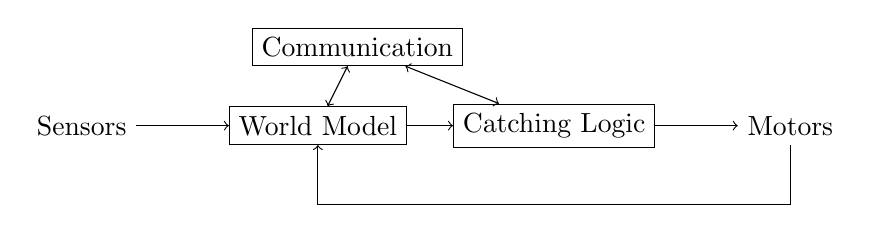
\begin{tikzpicture}
		\node (sensors) at (0, 0) { Sensors };
		\node (motors) at (9, 0) { Motors };
		\node[rectangle,draw] (world) at (3, 0) { World Model };
		\node[rectangle,draw] (logic) at (6, 0) { Catching Logic };
		\node[rectangle,draw] (comms) at (3.5, 1) { Communication };

		\draw[->] (sensors) edge (world);
		\draw[->] (world) edge (logic);
		\draw[->] (logic) edge (motors);
		\draw[->] (motors) -- (9, -1) -- (3, -1) -- (world);
		\draw[<->] (world) edge (comms);
		\draw[<->] (logic) edge (comms);
	\end{tikzpicture}
	\caption{Interaction between components}
\end{figure}

\subsection*{Work distribution}
\begin{itemize}
	\item Ultrasonic mapping:
	\begin{itemize}
		\item Laurens
		\item Jeftha
	\end{itemize}
	\item Navigation:
	\begin{itemize}
		\item Koen
		\item Simone
	\end{itemize}
	\item Cross-generation (NXT, EV3) abstraction layer
	\begin{itemize}
		\item Koen
	\end{itemize}
	\item Communication and diagnostics
	\begin{itemize}
		\item Tom
	\end{itemize} 
\end{itemize}

\subsection*{Feasibility considerations}
We have used the ultrasonic sensor in the past, but we were disappointed with the accuracy and consistency of the data. This year, we will attempt to factor this uncertainty into a map of the environment using a probabilistic model. We believe this will greatly improve accuracy.

To further minimize risk, we refrain from specifying the catching mechanism our robots will employ in this proposal. This way, we can adjust the difficulty of our project accordingly with our progress throughout the semester.

Furthermore, we will use Java instead of the default NXC language to ease the development process with obect-oriented features and LeJOS libraries.

\subsection*{Possible extensions}
\begin{itemize}
	\item More advanced catching mechanisms
	\item Voting on targets 
\end{itemize}

\subsection*{Other comments}
Last year we attempted a similar project, but failed. This was mostly due to the lack of reliable sensor information and incomplete/malfunctioning equipment and tooling. We have described a number of measures to solve these problems and are confident we can deliver a working prototype this year.

\end{document}
